\clearpage
\graphicspath{{./lib/error_correction/figures/}}
\section{Error correction}

\begin{tcolorbox}	
	\begin{tabular}{p{2.75cm} p{0.2cm} p{10.5cm}} 	
        \textbf{Header Files}    &:& error\_correction\_*.h \\
		\textbf{Source Files}    &:& error\_correction\_*.cpp \\
        \textbf{Version}         &:& 20190410 (Andoni Santos)
	\end{tabular}
\end{tcolorbox}

\maketitle
This block is used to correct the errors in the reconciled keys shared by two
parties in a quantum key distribution protocol. It currently implements the
Cascade error correction method, which resorts to iteratively exchanging
the parities of subsets from the sifted key in order to find errors.


% \begin{multicols}{3}
% \begin{enumerate}
% 	\item Random
% 	\item PseudoRandom
% 	\item DeterministicCyclic
% 	\item DeterministicAppendZeros
%     \item AsciiFileAppendZeros
%     \item AsciiFileCyclic
% \end{enumerate}
% \end{multicols}

\subsection*{Signals}

If errorCorrectionRole is Alice:

\begin{table}[h]
	%\centering
	\begin{tabular}{|c|l|}
		\hline
		\textbf{Number of Input Signals} & 5 \\ \hline
        \textbf{Type of Input Signals} & Binary,
        TimeDiscreteAmplitudeContinuousReal,\\
        & TimeDiscreteAmplitudeContinuousReal,\\
		& TimeDiscreteAmplitudeContinuousReal,\\
		& TimeDiscreteAmplitudeContinuousReal \\ \hline
    	\textbf{Number of Output Signals} & 2 \ \\ \hline
        \textbf{Type of Output Signals} & Binary, TimeDiscreteAmplitudeContinuousReal \\ \hline
	\end{tabular}
	\caption{Error correction signals - Alice}
	\label{table:bin_sour_signals}
\end{table}

If errorCorrectionRole is Bob:

\begin{table}[h]
	%\centering
	\begin{tabular}{|c|l|}
		\hline
		\textbf{Number of Input Signals} & 3 \\ \hline
		\textbf{Type of Input Signals} & Binary, TimeDiscreteAmplitudeContinuousReal\\
		& TimeDiscreteAmplitudeContinuousReal \\ \hline
    	\textbf{Number of Output Signals} & 4 \ \\ \hline
		\textbf{Type of Output Signals} & Binary, TimeDiscreteAmplitudeContinuousReal\\
		& TimeDiscreteAmplitudeContinuousReal \\
		& TimeDiscreteAmplitudeContinuousReal \\ \hline
	\end{tabular}
	\caption{Error correction signals - Bob}
	\label{table:bin_sour_signals}
\end{table}


\subsection*{Input Parameters}

\begin{table}[h]
	\centering
	\begin{tabular}{|c|c|p{60mm}|c|ccp{60mm}}
		\cline{1-4}
		\textbf{Parameter} & \textbf{Type} & \textbf{Values} &   \textbf{Default} \\ \cline{1-4}
		errorCorrectionRole & error\_correction\_role & \{ Alice, Bob, Undefined
		\} & Undefined \\ \cline{1-4}
		BER &  t\_real & [0,1] & 0 \\\cline{1-4}
		minimumBER & t\_real & >0 & 0.005 \\\cline{1-4}
		partitionSize & t\_integer & >= 6 & 10 \\\cline{1-4}
		numPasses & t\_integer & >= 1 & 4 \\\cline{1-4}
		doubleWindowSize & bool & \{ true, false \} & true \\\cline{1-4}
		minimumSyndromeSize & t\_integer & >= partitionSize & 10000 \\\cline{1-4}
		maximumSyndromeSize & t\_integer & >= minimumSyndromeSize & 10000 \\\cline{1-4}
		% mode & string & Random, PseudoRandom, DeterministicCyclic, DeterministicAppendZeros, AsciiFileAppendZeros, AsciiFileCyclic & PseudoRandom \\ \cline{1-4}
		% probabilityOfZero & real & $\in$ [0,1] & 0.5 \\ \cline{1-4}
		% patternLength & int &  Any natural number & 7 \\ \cline{1-4}
		% bitStream & string & sequence of 0's and 1's & 0100011101010101 \\ \cline{1-4}
		% numberOfBits & long int & any & -1 \\ \cline{1-4}
		% bitPeriod & double & any & $1.0/100e9$ \\ \cline{1-4}
        % asciiFilePath & string & any & ``file\_input\_data.txt" \\ \cline{1-4}
	\end{tabular}
	\caption{Error correction input parameters}
	\label{table:error_corr_in_par}
\end{table}

\subsection*{Methods}
ErrorCorrection(initializer\_list<Signal*> InputSig, initializer\_list<Signal*> OutputSig) : Block(InputSig, OutputSig) {};
\bigbreak
initialize(void);
\bigbreak
runBlock(void);
\bigbreak
setErrorCorrectionRole(error\_correction\_role role)
\bigbreak
setPartitionSize(t\_integer\ wsz)
\bigbreak
setBer(t\_real berValue)
\bigbreak
setNumberOfPasses(t\_integer np)
\bigbreak
setDoublePartitionSize(bool db)
\bigbreak
setMaximumSyndromeSize(t\_integer maxss)
\bigbreak
setMinimumSyndromeSize(t\_integer minss)
\bigbreak
setMinimumNumberOfPartitions(t\_integer mnp)
\bigbreak
getInputBits(void)
\bigbreak
getOutputBits(void)
\bigbreak
getNumberOfExchangedParities(void)


\subsection*{Functional description}

% The \textit{mode} parameter allows the user to select between one of the four operation modes of the binary source.

% \subparagraph*{Random Mode}
% Generates a 0 with probability \textit{probabilityOfZero} and a 1 with probability 1-\textit{probabilityOfZero}.

% \subparagraph*{Pseudorandom Mode}
% Generates a pseudorandom sequence with period $2^\textit{patternLength}-1$.

% \subparagraph*{DeterministicCyclic Mode}
% Generates the sequence of 0's and 1's specified by \textit{bitStream} and then repeats it.

% \subparagraph*{DeterministicAppendZeros Mode}
% Generates the sequence of 0's and 1's specified by \textit{bitStream} and then it fills the rest of the buffer space with zeros.



% \subsection*{Input Signals}


% \subparagraph*{Number:} 0

% \subparagraph*{Type:} Binary (DiscreteTimeDiscreteAmplitude)

% \subsection*{Output Signals}

% \subparagraph*{Number:} 1 or more

% \subparagraph*{Type:} Binary (DiscreteTimeDiscreteAmplitude)

% \subsection*{Illustrative Examples}

% \paragraph*{Random Mode}

% \paragraph*{PseudoRandom Mode}
% Consider a pseudorandom sequence with \textit{patternLength}=3 which contains a total of 7 ($2^3-1$) bits. In this sequence it is possible to find every combination of 0's and 1's that compose a 3 bit long subsequence with the exception of $000$. For this example the possible subsequences are $010$, $110$, $101$, $100$, $111$, $001$ and $100$ (they appear in figure \ref{BinarySequenceN3} numbered in this order). Some of these require wrap.

% % \begin{figure}[h]
% % 	\centering
% % 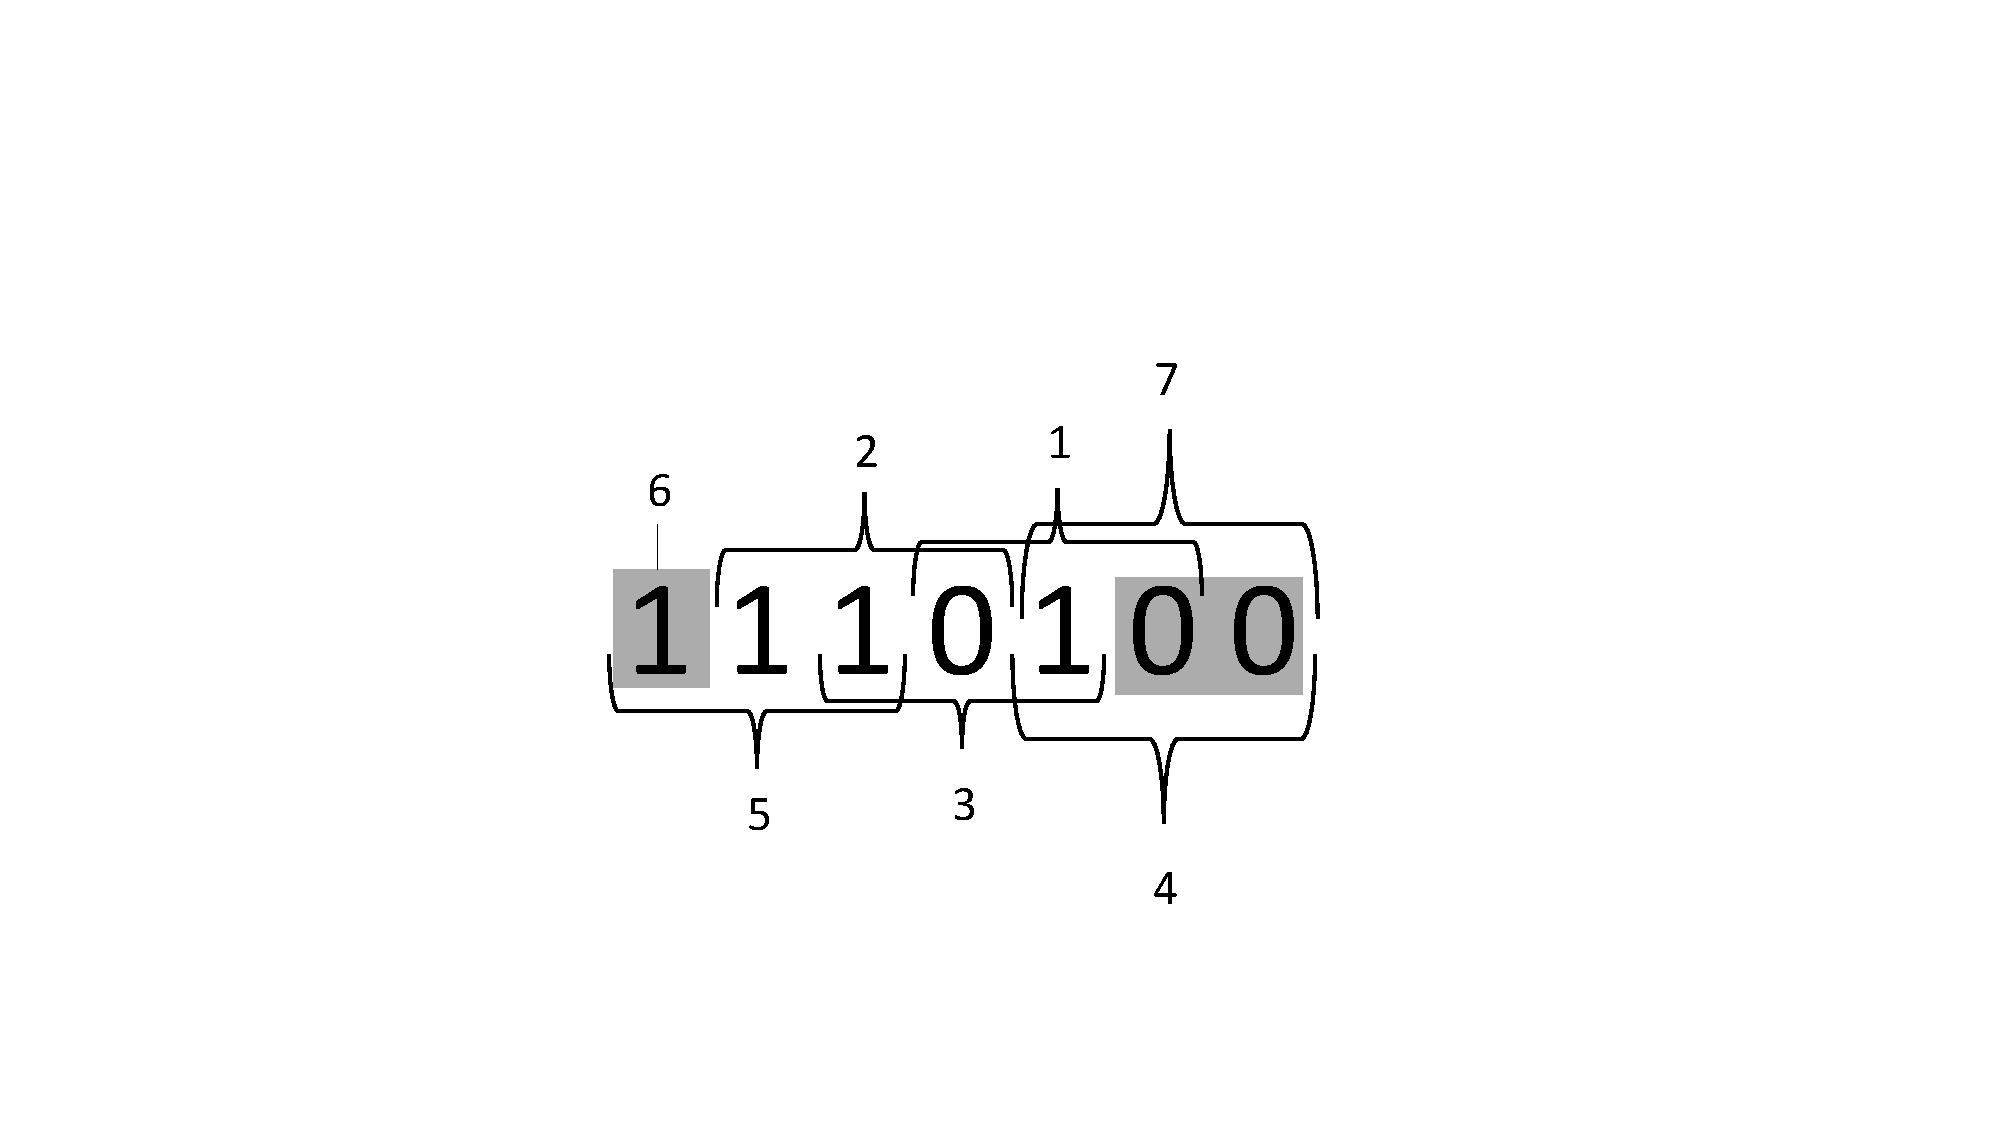
\includegraphics[width=\textwidth]{BinarySequenceN3.pdf}
% % \caption{Example of a pseudorandom sequence with a pattern length equal to 3.}\label{BinarySequenceN3}
% % \end{figure}

% \paragraph*{DeterministicCyclic Mode}

% Take the \textit{bit stream} '0100011101010101'. The generated binary signal is displayed in.

% \paragraph*{DeterministicAppendZeros Mode}

% Take the \textit{bit stream} '0100011101010101'. The generated binary signal is displayed in \ref{MQAM1_DeterministAppendZeros}.

% % \begin{figure}
% % 	\centering
% % 	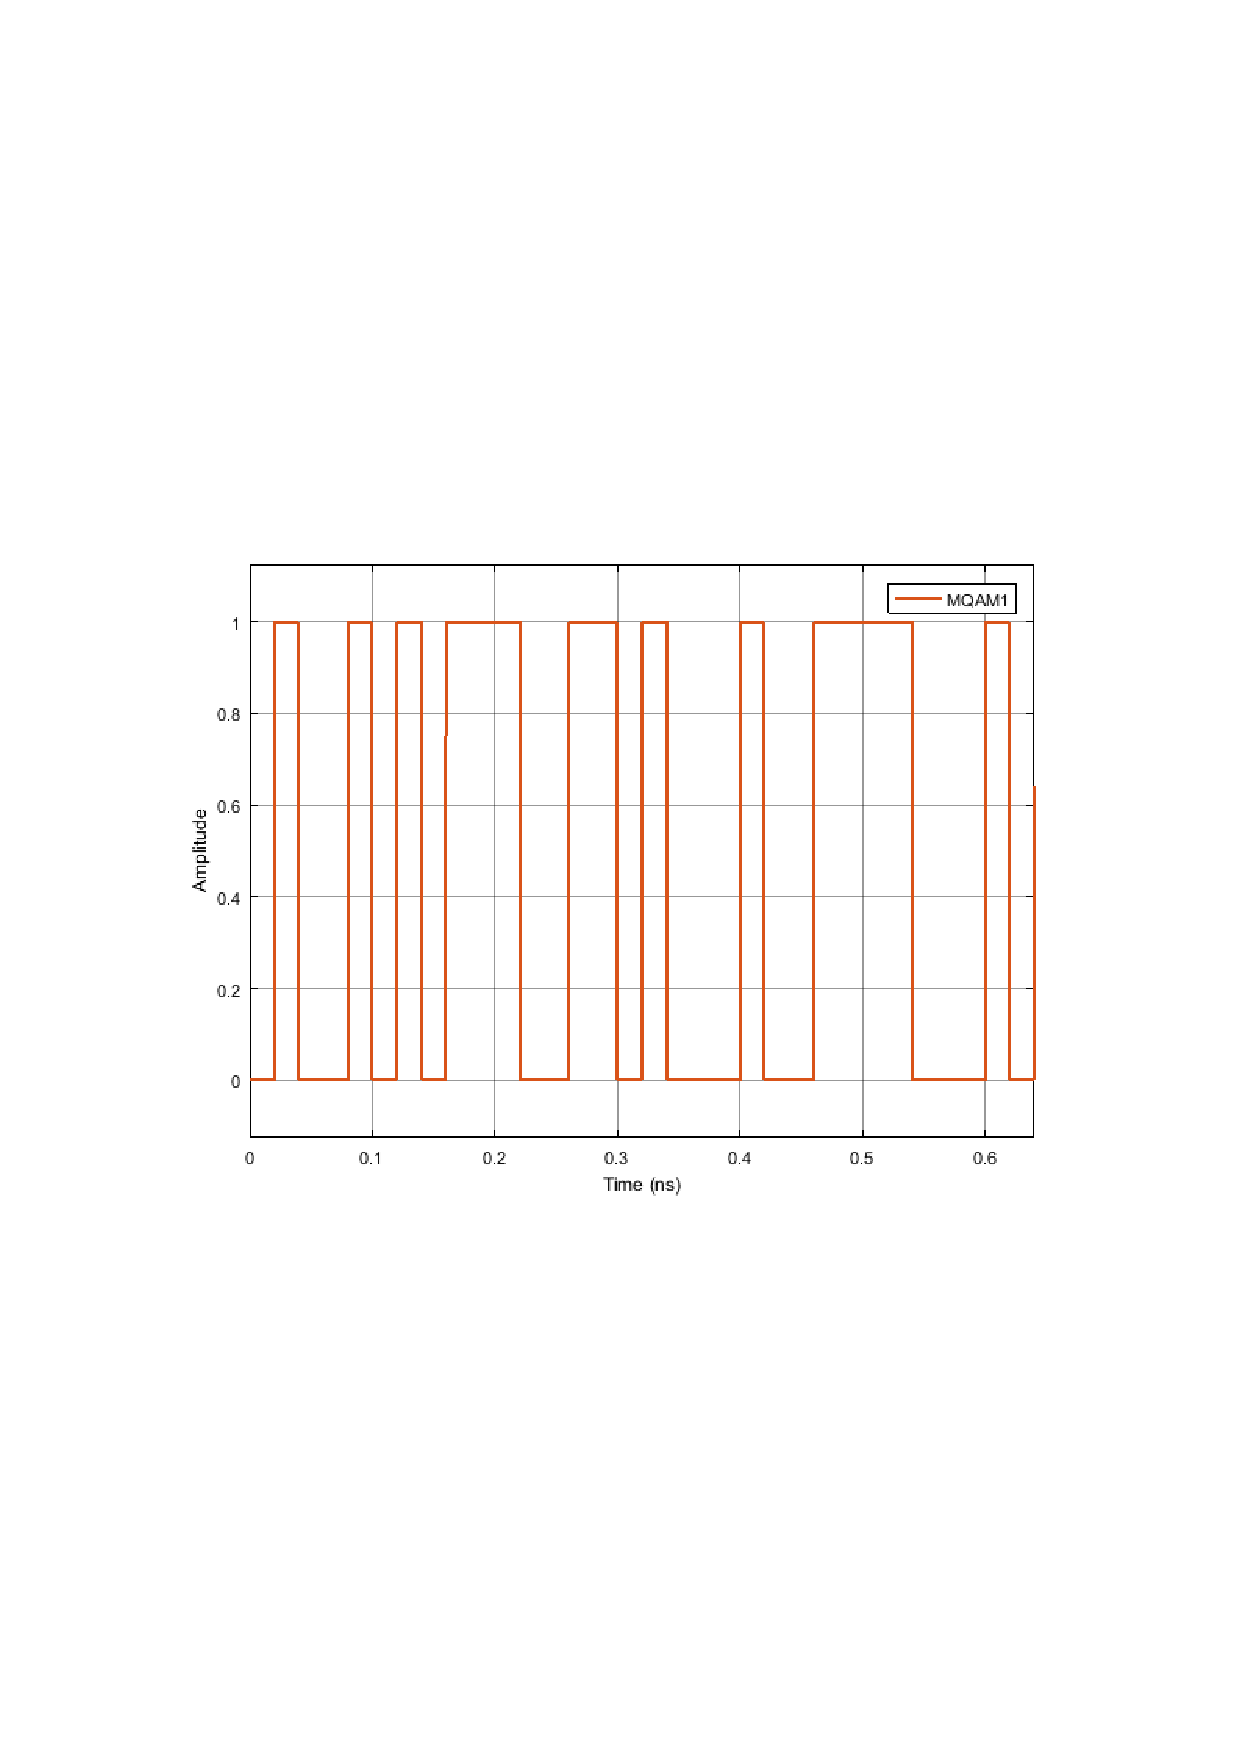
\includegraphics[clip, trim=0.5cm 9cm 0.5cm 9cm, width=\textwidth]{BinarySource_output.pdf}
	
% % 	\caption{Binary signal generated by the block operating in the \textit{Deterministic Append Zeros} mode with a binary sequence 01000...}\label{MQAM1_DeterministAppendZeros}
% % \end{figure}

\subsection*{Suggestions for future improvement}

% Currently, the number and type of signals is fixed, and cannot easily be
% adapted. In the future, this could be changed to allow easily adapting the
% message processors to other situations. In order to do that, it should be
% possible to choose a given number of signals and define the desired type for
% each of them.

